% szablon sprawozdania z dnia 2021-04-08
\documentclass{article} % mwart , article
\usepackage[polish]{babel}
\usepackage[utf8]{inputenc}	
\usepackage{polski}	
\usepackage[T1]{fontenc}
\frenchspacing	
\usepackage{indentfirst}
% PAKIETY DO MODYFIKACJI SRONY
\usepackage{fancybox} 
\usepackage{geometry}
\geometry{
	total={170mm,240mm},
	left=20mm,
	top=20mm,
}
% TABELA
\usepackage{multirow}
\usepackage{graphicx}
\usepackage{array}
\usepackage{makecell}
% INNE
\usepackage{color, colortbl}
\definecolor{Gray}{gray}{0.9}
\usepackage{lipsum}
% USTAWIENIA SUBSECTION
\usepackage[compact]{titlesec}
\titleformat{\subsection}[runin]
{\normalfont\large\bfseries}{\thesubsection}{1em}{}[{\\[0,5em]}]
\titlespacing*{\subsection}{1cm}{1em}{0em}
% dodanie FORCEINDENT
\newcommand{\forceindent}{\leavevmode{\parindent=1cm\indent}} %
\setlength{\parindent}{1cm}


% TYTUŁ, DATY ORAZ DANE OSOBY OPRACOWUJĄCEJ SPRAWOZDANIE
\def\AuthorFirstName{DARIUSZ}
\def\AuthorLastName{KOZA}
\def\Title{Zapoznanie z zasadami bezpieczeństwa obowiązującymi \\w laboratorium, potwierdzenie odbycia instruktażu. \\ Wprowadzenie do LV, instalacja urządzeń,\\ Nawigacja w LabVIEW.}
\def\DateOfExecution{2022-04-08}
\def\DateOfDeliver{2022-04-09}
%
%
\begin{document}	
	%\fancypage{\setlength{\fboxsep}{0pt}\doublebox}{}	
	\noindent
	\def\arraystretch{1.5} \small
% TABELA Z DANYMI
	\begin{table}
		\resizebox{\textwidth}{!}{\begin{tabular}{|p{2cm}|p{4cm}|p{3.5cm}|p{3cm}|l|}
		\hline 
		\multirow{4}{*}{\makecell[l]{
\includegraphics[width=2cm]{image/ModLogoPO}\\
\includegraphics[width=2cm]{image/ModLogoWE}}} & PRZEDMIOT: & \multicolumn{3}{l|}{ \makecell[l]{\noalign{\vskip3pt}PRZEDMIOT WYBIERALNY V:\\ NARZ\k{E}DZIA INFORMATYCZNE W PRAKTYCE \\IN\.{Z}YNIERSKIEJ}}\tabularnewline
		\cline{2-5} \cline{3-5} \cline{4-5} \cline{5-5} 
		& KIERUNEK STUDIÓW: & ELEKTROTECHNIKA & ROK STUDIÓW: & II\tabularnewline
		\cline{2-5} \cline{3-5} \cline{4-5} \cline{5-5} 
		& ROK AKADEMICKI: & 2021/2022 & SEMESTR: & 4 \tabularnewline
		\cline{2-5} \cline{3-5} \cline{4-5} \cline{5-5} 
		& TEMAT: & \multicolumn{3}{l|}{\makecell[l]{\noalign{\vskip3pt} \Title }}\tabularnewline
		\hline 
		IMI\k{E}: & \textbf{\AuthorFirstName} & \multicolumn{2}{l|}{DATA WYKONANIA \'{C}WICZENIA: }  & \DateOfExecution \tabularnewline
		\hline 
		NAZWISKO: & \textbf{\AuthorLastName} & \multicolumn{2}{l|}{DATA ODDANIA SPRAWOZDANIA:} & \DateOfDeliver \tabularnewline
		\hline 
		OCENA: & DATA: & \multicolumn{3}{l|}{UWAGI:}\tabularnewline
		\hline \rowcolor{Gray}
		{\makecell[l]{ \\ \\ \\ \\}}&  & \multicolumn{3}{l|}{}\tabularnewline
		\hline 
		\end{tabular}}
	\end{table}
% POCZĄTEK SPRAWOZDANIA
	
	\section{Zadanie 1}
		\subsection{Cel ćwiczenia}
		
			Celem ćwiczenia jest zapoznanie się z tworzeniem plików tekstowych w środowisku LATEX.
		
		\subsection{Algorytm programu}
		\begin{figure}
		
			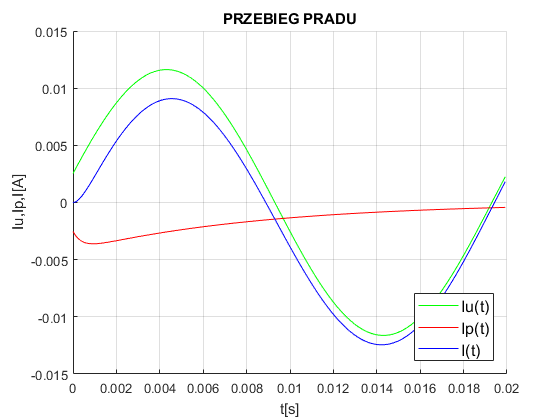
\includegraphics[width=12cm]{91.png}
				\caption{Podpis pod rysunkiem}
		\end{figure}	
	
		\subsection{Opis programu}
		
		\subsection{Podsumowanie}
		
	\section{Zadanie 2}
		\subsection{Cel ćwiczenia}
		
		\subsection{Algorytm programu}
				
		\subsection{Opis programu}
			
		\subsection{Podsumowanie}
					
	
\end{document}	